%%%%%%%%%%%%%%%%%%%%%%%%%%%%%%%%%%%%%%%%%
% The Legrand Orange Book
% LaTeX Template
% Version 2.2 (30/3/17)
%
% This template has been downloaded from:
% http://www.LaTeXTemplates.com
%
% Original author:
% Mathias Legrand (legrand.mathias@gmail.com) with modifications by:
% Vel (vel@latextemplates.com)
% modified slightly by the iGEM team TU Dresden 2017
%
% License:
% cc BY-NC-SA 3.0 (http://creativecommons.org/licenses/by-nc-sa/3.0/)
%
% Compiling this template:
% This template uses biber for its bibliography and makeindex for its index.
% When you first open the template, compile it from the command line with the 
% commands below to make sure your LaTeX distribution is configured correctly:
%
% 1) pdflatex GoGreenGuide
% 2) makeindex GoGreenGuide.idx -s StyleInd.ist
% 3) biber GoGreenGuide
% 4) pdflatex GoGreenGuide x 2
%
% After this, when you wish to update the bibliography/index use the appropriate
% command above and make sure to compile with pdflatex several times 
% afterwards to propagate your changes to the document.
%
% This template also uses a number of packages which may need to be
% updated to the newest versions for the template to compile. It is strongly
% recommended you update your LaTeX distribution if you have any
% compilation errors.
%
% Important note:
% Chapter heading images should have a 2:1 width:height ratio,
% e.g. 920px width and 460px height.
%
%%%%%%%%%%%%%%%%%%%%%%%%%%%%%%%%%%%%%%%%%

%----------------------------------------------------------------------------------------
%	PACKAGES AND OTHER DOCUMENT CONFIGURATIONS
%----------------------------------------------------------------------------------------

\documentclass[11pt,fleqn,openany]{book} % Default font size and left-justified equations

%%%%%%%%%%%%%%%%%%%%%%%%%%%%%%%%%%%%%%%%%
% The Legrand Orange Book
% Structural Definitions File
% Version 2.0 (9/2/15)
%
% Original author:
% Mathias Legrand (legrand.mathias@gmail.com) with modifications by:
% Vel (vel@latextemplates.com)
% 
% This file has been downloaded from:
% http://www.LaTeXTemplates.com
%
% License:
% CC BY-NC-SA 3.0 (http://creativecommons.org/licenses/by-nc-sa/3.0/)
%
%%%%%%%%%%%%%%%%%%%%%%%%%%%%%%%%%%%%%%%%%

%----------------------------------------------------------------------------------------
%	VARIOUS REQUIRED PACKAGES AND CONFIGURATIONS
%----------------------------------------------------------------------------------------

\usepackage[top=3cm,bottom=3cm,left=3cm,right=3cm,headsep=10pt,a4paper]{geometry} % Page margins

\usepackage{graphicx} % Required for including pictures
\graphicspath{{Images/}} % Specifies the directory where pictures are stored

\usepackage{lipsum} % Inserts dummy text

\usepackage{tikz} % Required for drawing custom shapes

\usepackage[english]{babel} % English language/hyphenation

\usepackage{enumitem} % Customize lists
\setlist{nolistsep} % Reduce spacing between bullet points and numbered lists

\usepackage{booktabs} % Required for nicer horizontal rules in tables

\usepackage{xcolor} % Required for specifying colors by name
\definecolor{ocre}{RGB}{17,121,34} % Define the orange color used for highlighting throughout the book <-- changed to green

%----------------------------------------------------------------------------------------
%	FONTS
%----------------------------------------------------------------------------------------

\usepackage{avant} % Use the Avantgarde font for headings
%\usepackage{times} % Use the Times font for headings
\usepackage{mathptmx} % Use the Adobe Times Roman as the default text font together with math symbols from the Sym­bol, Chancery and Com­puter Modern fonts

\usepackage{microtype} % Slightly tweak font spacing for aesthetics
\usepackage[utf8]{inputenc} % Required for including letters with accents
\usepackage[T1]{fontenc} % Use 8-bit encoding that has 256 glyphs

%----------------------------------------------------------------------------------------
%	BIBLIOGRAPHY AND INDEX
%----------------------------------------------------------------------------------------

\usepackage[style=alphabetic,citestyle=numeric,sorting=nyt,sortcites=true,autopunct=true,babel=hyphen,hyperref=true,abbreviate=false,backref=true,backend=biber]{biblatex}
\addbibresource{bibliography.bib} % BibTeX bibliography file
\defbibheading{bibempty}{}

\usepackage{calc} % For simpler calculation - used for spacing the index letter headings correctly
\usepackage{makeidx} % Required to make an index
\makeindex % Tells LaTeX to create the files required for indexing

%----------------------------------------------------------------------------------------
%	MAIN TABLE OF CONTENTS
%----------------------------------------------------------------------------------------

\usepackage{titletoc} % Required for manipulating the table of contents

\contentsmargin{0cm} % Removes the default margin

% Part text styling
\titlecontents{part}[0cm]
{\addvspace{20pt}\centering\large\bfseries}
{}
{}
{}

% Chapter text styling
\titlecontents{chapter}[1.25cm] % Indentation
{\addvspace{12pt}\large\sffamily\bfseries} % Spacing and font options for chapters
{\color{ocre!60}\contentslabel[\Large\thecontentslabel]{1.25cm}\color{ocre}} % Chapter number
{\color{ocre}}  
{\color{ocre!60}\normalsize\;\titlerule*[.5pc]{.}\;\thecontentspage} % Page number

% Section text styling
\titlecontents{section}[1.25cm] % Indentation
{\addvspace{3pt}\sffamily\bfseries} % Spacing and font options for sections
{\contentslabel[\thecontentslabel]{1.25cm}} % Section number
{}
{\hfill\color{black}\thecontentspage} % Page number
[]

% Subsection text styling
\titlecontents{subsection}[1.25cm] % Indentation
{\addvspace{1pt}\sffamily\small} % Spacing and font options for subsections
{\contentslabel[\thecontentslabel]{1.25cm}} % Subsection number
{}
{\ \titlerule*[.5pc]{.}\;\thecontentspage} % Page number
[]

% List of figures
\titlecontents{figure}[0em]
{\addvspace{-5pt}\sffamily}
{\thecontentslabel\hspace*{1em}}
{}
{\ \titlerule*[.5pc]{.}\;\thecontentspage}
[]

% List of tables
\titlecontents{table}[0em]
{\addvspace{-5pt}\sffamily}
{\thecontentslabel\hspace*{1em}}
{}
{\ \titlerule*[.5pc]{.}\;\thecontentspage}
[]

%----------------------------------------------------------------------------------------
%	MINI TABLE OF CONTENTS IN PART HEADS
%----------------------------------------------------------------------------------------

% Chapter text styling
\titlecontents{lchapter}[0em] % Indenting
{\addvspace{15pt}\large\sffamily\bfseries} % Spacing and font options for chapters
{\color{ocre}\contentslabel[\Large\thecontentslabel]{1.25cm}\color{ocre}} % Chapter number
{}  
{\color{ocre}\normalsize\sffamily\bfseries\;\titlerule*[.5pc]{.}\;\thecontentspage} % Page number

% Section text styling
\titlecontents{lsection}[0em] % Indenting
{\sffamily\small} % Spacing and font options for sections
{\contentslabel[\thecontentslabel]{1.25cm}} % Section number
{}
{}

% Subsection text styling
\titlecontents{lsubsection}[.5em] % Indentation
{\normalfont\footnotesize\sffamily} % Font settings
{}
{}
{}

%----------------------------------------------------------------------------------------
%	PAGE HEADERS
%----------------------------------------------------------------------------------------

\usepackage{fancyhdr} % Required for header and footer configuration

\pagestyle{fancy}
\renewcommand{\chaptermark}[1]{\markboth{\sffamily\normalsize\bfseries\chaptername\ \thechapter.\ #1}{}} % Chapter text font settings
\renewcommand{\sectionmark}[1]{\markright{\sffamily\normalsize\thesection\hspace{5pt}#1}{}} % Section text font settings
\fancyhf{} \fancyhead[LE,RO]{\sffamily\normalsize\thepage} % Font setting for the page number in the header
\fancyhead[LO]{\rightmark} % Print the nearest section name on the left side of odd pages
\fancyhead[RE]{\leftmark} % Print the current chapter name on the right side of even pages
\renewcommand{\headrulewidth}{0.5pt} % Width of the rule under the header
\addtolength{\headheight}{2.5pt} % Increase the spacing around the header slightly
\renewcommand{\footrulewidth}{0pt} % Removes the rule in the footer
\fancypagestyle{plain}{\fancyhead{}\renewcommand{\headrulewidth}{0pt}} % Style for when a plain pagestyle is specified

% Removes the header from odd empty pages at the end of chapters
\makeatletter
\renewcommand{\cleardoublepage}{
	\clearpage\ifodd\c@page\else
	\hbox{}
	\vspace*{\fill}
	\thispagestyle{empty}
	\newpage
	\fi}

%----------------------------------------------------------------------------------------
%	THEOREM STYLES
%----------------------------------------------------------------------------------------

\usepackage{amsmath,amsfonts,amssymb,amsthm} % For math equations, theorems, symbols, etc

\newcommand{\intoo}[2]{\mathopen{]}#1\,;#2\mathclose{[}}
\newcommand{\ud}{\mathop{\mathrm{{}d}}\mathopen{}}
\newcommand{\intff}[2]{\mathopen{[}#1\,;#2\mathclose{]}}
\newtheorem{notation}{Notation}[chapter]

% Boxed/framed environments
\newtheoremstyle{ocrenumbox}% % Theorem style name
{0pt}% Space above
{0pt}% Space below
{\normalfont}% % Body font
{}% Indent amount
{\small\bf\sffamily\color{ocre}}% % Theorem head font
{\;}% Punctuation after theorem head
{0.25em}% Space after theorem head
{\small\sffamily\color{ocre}\thmname{#1}\nobreakspace\thmnumber{\@ifnotempty{#1}{}\@upn{#2}}% Theorem text (e.g. Theorem 2.1)
	\thmnote{\nobreakspace\the\thm@notefont\sffamily\bfseries\color{black}---\nobreakspace#3.}} % Optional theorem note
\renewcommand{\qedsymbol}{$\blacksquare$}% Optional qed square

\newtheoremstyle{blacknumex}% Theorem style name
{5pt}% Space above
{5pt}% Space below
{\normalfont}% Body font
{} % Indent amount
{\small\bf\sffamily}% Theorem head font
{\;}% Punctuation after theorem head
{0.25em}% Space after theorem head
{\small\sffamily{\tiny\ensuremath{\blacksquare}}\nobreakspace\thmname{#1}\nobreakspace\thmnumber{\@ifnotempty{#1}{}\@upn{#2}}% Theorem text (e.g. Theorem 2.1)
	\thmnote{\nobreakspace\the\thm@notefont\sffamily\bfseries---\nobreakspace#3.}}% Optional theorem note

\newtheoremstyle{blacknumbox} % Theorem style name
{0pt}% Space above
{0pt}% Space below
{\normalfont}% Body font
{}% Indent amount
{\small\bf\sffamily}% Theorem head font
{\;}% Punctuation after theorem head
{0.25em}% Space after theorem head
{\small\sffamily\thmname{#1}\nobreakspace\thmnumber{\@ifnotempty{#1}{}\@upn{#2}}% Theorem text (e.g. Theorem 2.1)
	\thmnote{\nobreakspace\the\thm@notefont\sffamily\bfseries---\nobreakspace#3.}}% Optional theorem note

% Non-boxed/non-framed environments
\newtheoremstyle{ocrenum}% % Theorem style name
{5pt}% Space above
{5pt}% Space below
{\normalfont}% % Body font
{}% Indent amount
{\small\bf\sffamily\color{ocre}}% % Theorem head font
{\;}% Punctuation after theorem head
{0.25em}% Space after theorem head
{\small\sffamily\color{ocre}\thmname{#1}\nobreakspace\thmnumber{\@ifnotempty{#1}{}\@upn{#2}}% Theorem text (e.g. Theorem 2.1)
	\thmnote{\nobreakspace\the\thm@notefont\sffamily\bfseries\color{black}---\nobreakspace#3.}} % Optional theorem note
\renewcommand{\qedsymbol}{$\blacksquare$}% Optional qed square
\makeatother

% Defines the theorem text style for each type of theorem to one of the three styles above
\newcounter{dummy} 
\numberwithin{dummy}{section}
\theoremstyle{ocrenumbox}
\newtheorem{theoremeT}[dummy]{Theorem}
\newtheorem{problem}{Problem}[chapter]
\newtheorem{exerciseT}{Exercise}[chapter]
\theoremstyle{blacknumex}
\newtheorem{exampleT}{Example}[chapter]
\theoremstyle{blacknumbox}
\newtheorem{vocabulary}{Vocabulary}[chapter]
\newtheorem{definitionT}{Definition}[section]
\newtheorem{corollaryT}[dummy]{Corollary}
\theoremstyle{ocrenum}
\newtheorem{proposition}[dummy]{Proposition}

%----------------------------------------------------------------------------------------
%	DEFINITION OF COLORED BOXES
%----------------------------------------------------------------------------------------

\RequirePackage[framemethod=default]{mdframed} % Required for creating the theorem, definition, exercise and corollary boxes

% Theorem box
\newmdenv[skipabove=7pt,
skipbelow=7pt,
backgroundcolor=black!5,
linecolor=ocre,
innerleftmargin=5pt,
innerrightmargin=5pt,
innertopmargin=5pt,
leftmargin=0cm,
rightmargin=0cm,
innerbottommargin=5pt]{tBox}

% Exercise box	  
\newmdenv[skipabove=7pt,
skipbelow=7pt,
rightline=false,
leftline=true,
topline=false,
bottomline=false,
backgroundcolor=ocre!10,
linecolor=ocre,
innerleftmargin=5pt,
innerrightmargin=5pt,
innertopmargin=5pt,
innerbottommargin=5pt,
leftmargin=0cm,
rightmargin=0cm,
linewidth=4pt]{eBox}	

% Definition box
\newmdenv[skipabove=7pt,
skipbelow=7pt,
rightline=false,
leftline=true,
topline=false,
bottomline=false,
linecolor=ocre,
innerleftmargin=5pt,
innerrightmargin=5pt,
innertopmargin=0pt,
leftmargin=0cm,
rightmargin=0cm,
linewidth=4pt,
innerbottommargin=0pt]{dBox}	

% Corollary box
\newmdenv[skipabove=7pt,
skipbelow=7pt,
rightline=false,
leftline=true,
topline=false,
bottomline=false,
linecolor=gray,
backgroundcolor=black!5,
innerleftmargin=5pt,
innerrightmargin=5pt,
innertopmargin=5pt,
leftmargin=0cm,
rightmargin=0cm,
linewidth=4pt,
innerbottommargin=5pt]{cBox}

% Creates an environment for each type of theorem and assigns it a theorem text style from the "Theorem Styles" section above and a colored box from above
\newenvironment{theorem}{\begin{tBox}\begin{theoremeT}}{\end{theoremeT}\end{tBox}}
\newenvironment{exercise}{\begin{eBox}\begin{exerciseT}}{\hfill{\color{ocre}\tiny\ensuremath{\blacksquare}}\end{exerciseT}\end{eBox}}				  
\newenvironment{definition}{\begin{dBox}\begin{definitionT}}{\end{definitionT}\end{dBox}}	
\newenvironment{example}{\begin{exampleT}}{\hfill{\tiny\ensuremath{\blacksquare}}\end{exampleT}}		
\newenvironment{corollary}{\begin{cBox}\begin{corollaryT}}{\end{corollaryT}\end{cBox}}	

%----------------------------------------------------------------------------------------
%	REMARK ENVIRONMENT
%----------------------------------------------------------------------------------------

\newenvironment{remark}{\par\vspace{10pt}\small % Vertical white space above the remark and smaller font size
	\begin{list}{}{
			\leftmargin=35pt % Indentation on the left
			\rightmargin=25pt}\item\ignorespaces % Indentation on the right
		\makebox[-2.5pt]{\begin{tikzpicture}[overlay]
			\node[draw=ocre!60,line width=1pt,circle,fill=ocre!25,font=\sffamily\bfseries,inner sep=2pt,outer sep=0pt] at (-15pt,0pt){\textcolor{ocre}{R}};\end{tikzpicture}} % Orange R in a circle
		\advance\baselineskip -1pt}{\end{list}\vskip5pt} % Tighter line spacing and white space after remark

%----------------------------------------------------------------------------------------
%	SECTION NUMBERING IN THE MARGIN
%----------------------------------------------------------------------------------------

\makeatletter
\renewcommand{\@seccntformat}[1]{\llap{\textcolor{ocre}{\csname the#1\endcsname}\hspace{1em}}}                    
\renewcommand{\section}{\@startsection{section}{1}{\z@}
	{-4ex \@plus -1ex \@minus -.4ex}
	{1ex \@plus.2ex }
	{\normalfont\large\sffamily\bfseries}}
\renewcommand{\subsection}{\@startsection {subsection}{2}{\z@}
	{-3ex \@plus -0.1ex \@minus -.4ex}
	{0.5ex \@plus.2ex }
	{\normalfont\sffamily\bfseries}}
\renewcommand{\subsubsection}{\@startsection {subsubsection}{3}{\z@}
	{-2ex \@plus -0.1ex \@minus -.2ex}
	{.2ex \@plus.2ex }
	{\normalfont\small\sffamily\bfseries}}                        
\renewcommand\paragraph{\@startsection{paragraph}{4}{\z@}
	{-2ex \@plus-.2ex \@minus .2ex}
	{.1ex}
	{\normalfont\small\sffamily\bfseries}}

%----------------------------------------------------------------------------------------
%	PART HEADINGS
%----------------------------------------------------------------------------------------

% numbered part in the table of contents
\newcommand{\@mypartnumtocformat}[2]{%
	\setlength\fboxsep{0pt}%
	\noindent\colorbox{ocre!20}{\strut\parbox[c][.7cm]{\ecart}{\color{ocre!70}\Large\sffamily\bfseries\centering#1}}\hskip\esp\colorbox{ocre!40}{\strut\parbox[c][.7cm]{\linewidth-\ecart-\esp}{\Large\sffamily\centering#2}}}%
%%%%%%%%%%%%%%%%%%%%%%%%%%%%%%%%%%
% unnumbered part in the table of contents
\newcommand{\@myparttocformat}[1]{%
	\setlength\fboxsep{0pt}%
	\noindent\colorbox{ocre!40}{\strut\parbox[c][.7cm]{\linewidth}{\Large\sffamily\centering#1}}}%
%%%%%%%%%%%%%%%%%%%%%%%%%%%%%%%%%%
\newlength\esp
\setlength\esp{4pt}
\newlength\ecart
\setlength\ecart{1.2cm-\esp}
\newcommand{\thepartimage}{}%
\newcommand{\partimage}[1]{\renewcommand{\thepartimage}{#1}}%
\def\@part[#1]#2{%
	\ifnum \c@secnumdepth >-2\relax%
	\refstepcounter{part}%
	\addcontentsline{toc}{part}{\texorpdfstring{\protect\@mypartnumtocformat{\thepart}{#1}}{\partname~\thepart\ ---\ #1}}
	\else%
	\addcontentsline{toc}{part}{\texorpdfstring{\protect\@myparttocformat{#1}}{#1}}%
	\fi%
	\startcontents%
	\markboth{}{}%
	{\thispagestyle{empty}%
		\begin{tikzpicture}[remember picture,overlay]%
		\node at (current page.north west){\begin{tikzpicture}[remember picture,overlay]%	
			\fill[ocre!20](0cm,0cm) rectangle (\paperwidth,-\paperheight);
			\node[anchor=north] at (4cm,-3.25cm){\color{ocre!40}\fontsize{220}{100}\sffamily\bfseries\thepart}; 
			\node[anchor=south east] at (\paperwidth-1cm,-\paperheight+1cm){\parbox[t][][t]{8.5cm}{
					\printcontents{l}{0}{\setcounter{tocdepth}{1}}%
				}};
				\node[anchor=north east] at (\paperwidth-1.5cm,-3.25cm){\parbox[t][][t]{15cm}{\strut\raggedleft\color{white}\fontsize{30}{30}\sffamily\bfseries#2}};
				\end{tikzpicture}};
		\end{tikzpicture}}%
		\@endpart}
	\def\@spart#1{%
		\startcontents%
		\phantomsection
		{\thispagestyle{empty}%
			\begin{tikzpicture}[remember picture,overlay]%
			\node at (current page.north west){\begin{tikzpicture}[remember picture,overlay]%	
				\fill[ocre!20](0cm,0cm) rectangle (\paperwidth,-\paperheight);
				\node[anchor=north east] at (\paperwidth-1.5cm,-3.25cm){\parbox[t][][t]{15cm}{\strut\raggedleft\color{white}\fontsize{30}{30}\sffamily\bfseries#1}};
				\end{tikzpicture}};
		\end{tikzpicture}}
		\addcontentsline{toc}{part}{\texorpdfstring{%
				\setlength\fboxsep{0pt}%
				\noindent\protect\colorbox{ocre!40}{\strut\protect\parbox[c][.7cm]{\linewidth}{\Large\sffamily\protect\centering #1\quad\mbox{}}}}{#1}}%
		\@endpart}
	\def\@endpart{\vfil\newpage
		\if@twoside
		\if@openright
		\null
		\thispagestyle{empty}%
		\newpage
		\fi
		\fi
		\if@tempswa
		\twocolumn
		\fi}
	
	%----------------------------------------------------------------------------------------
	%	CHAPTER HEADINGS
	%----------------------------------------------------------------------------------------
	
	% A switch to conditionally include a picture, implemented by  Christian Hupfer
	\newif\ifusechapterimage
	\usechapterimagetrue
	\newcommand{\thechapterimage}{}%
	\newcommand{\chapterimage}[1]{\ifusechapterimage\renewcommand{\thechapterimage}{#1}\fi}%
	\newcommand{\autodot}{.}
	\def\@makechapterhead#1{%
		{\parindent \z@ \raggedright \normalfont
			\ifnum \c@secnumdepth >\m@ne
			\if@mainmatter
			\begin{tikzpicture}[remember picture,overlay]
			\node at (current page.north west)
			{\begin{tikzpicture}[remember picture,overlay]
				\node[anchor=north west,inner sep=0pt] at (0,0) {\ifusechapterimage\includegraphics[width=\paperwidth]{\thechapterimage}\fi};
				\draw[anchor=west] (\Gm@lmargin,-9cm) node [line width=2pt,rounded corners=15pt,draw=ocre,fill=white,fill opacity=0.5,inner sep=15pt]{\strut\makebox[22cm]{}};
				\draw[anchor=west] (\Gm@lmargin+.3cm,-9.1cm) node {\huge\sffamily\bfseries\color{black}\thechapter\autodot~#1\strut};
				\end{tikzpicture}};
		\end{tikzpicture}
		\else
		\begin{tikzpicture}[remember picture,overlay]
		\node at (current page.north west)
		{\begin{tikzpicture}[remember picture,overlay]
			\node[anchor=north west,inner sep=0pt] at (0,0) {\ifusechapterimage\includegraphics[width=\paperwidth]{\thechapterimage}\fi};
			\draw[anchor=west] (\Gm@lmargin,-9cm) node [line width=2pt,rounded corners=15pt,draw=ocre,fill=white,fill opacity=0.5,inner sep=15pt]{\strut\makebox[22cm]{}};
			\draw[anchor=west] (\Gm@lmargin+.3cm,-9.1cm) node {\huge\sffamily\bfseries\color{black}#1\strut};
			\end{tikzpicture}};
	\end{tikzpicture}
	\fi\fi\par\vspace*{270\p@}}}

%-------------------------------------------

\def\@makeschapterhead#1{%
	\begin{tikzpicture}[remember picture,overlay]
	\node at (current page.north west)
	{\begin{tikzpicture}[remember picture,overlay]
		\node[anchor=north west,inner sep=0pt] at (0,0) {\ifusechapterimage\includegraphics[width=\paperwidth]{\thechapterimage}\fi};
		\draw[anchor=west] (\Gm@lmargin,-9cm) node [line width=2pt,rounded corners=15pt,draw=ocre,fill=white,fill opacity=0.5,inner sep=15pt]{\strut\makebox[22cm]{}};
		\draw[anchor=west] (\Gm@lmargin+.3cm,-9cm) node {\huge\sffamily\bfseries\color{black}#1\strut};
		\end{tikzpicture}};
\end{tikzpicture}
\par\vspace*{270\p@}}
\makeatother

%----------------------------------------------------------------------------------------
%	HYPERLINKS IN THE DOCUMENTS
%----------------------------------------------------------------------------------------

\usepackage{hyperref}
\hypersetup{hidelinks,backref=true,pagebackref=true,hyperindex=true,colorlinks=false,breaklinks=true,urlcolor= ocre,bookmarks=true,bookmarksopen=false,pdftitle={Title},pdfauthor={Author}}
\usepackage{bookmark}
\bookmarksetup{
	open,
	numbered,
	addtohook={%
		\ifnum\bookmarkget{level}=0 % chapter
		\bookmarksetup{bold}%
		\fi
		\ifnum\bookmarkget{level}=-1 % part
		\bookmarksetup{color=ocre,bold}%
		\fi
	}
}
 % Insert the formatting.tex file which contains the majority of the structure behind the template

%----------------------------------------------------------------------------------------

\begin{document}
	
	%----------------------------------------------------------------------------------------
	%	TITLE PAGE
	%----------------------------------------------------------------------------------------
	
	\begingroup
	\thispagestyle{empty}
	\begin{tikzpicture}[remember picture,overlay]
	\node[inner sep=0pt] (background) at (current page.center) {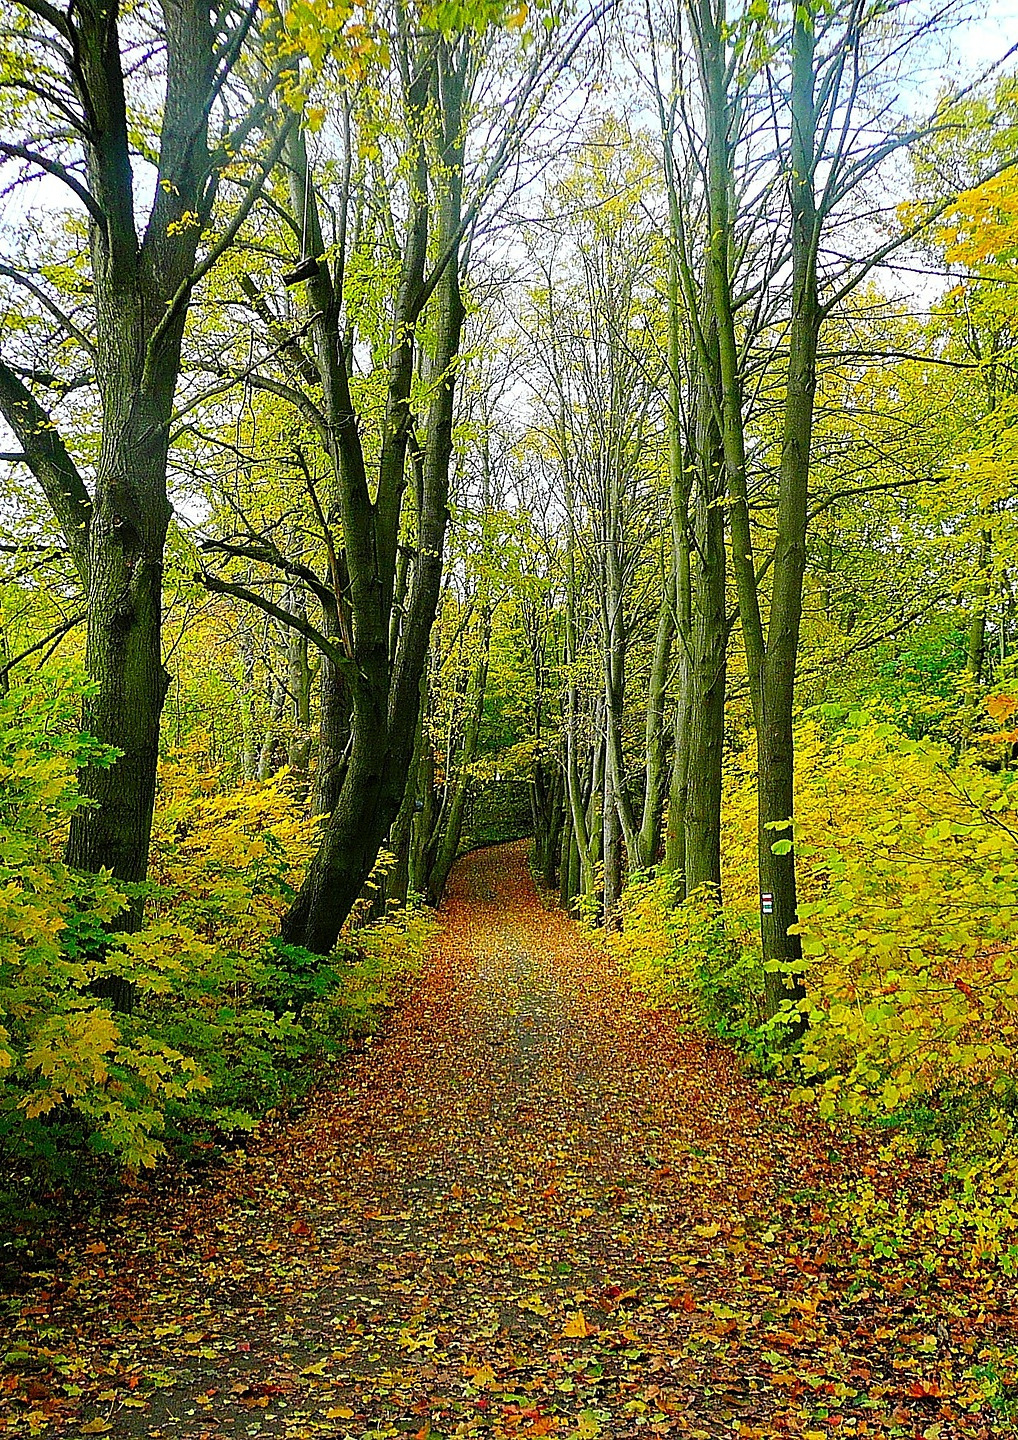
\includegraphics[width=\paperwidth]{background.jpg}};
	\draw ([yshift=7cm]current page.center) node [fill=ocre!40!white,fill opacity=0.6,text opacity=1,inner sep=2cm]{\Huge\centering\bfseries\sffamily\parbox[c][][t]{\paperwidth}{\centering GoGreenGuide\\[15pt] % Book title
			{\LARGE The Official iGEM goes green Guideline}\\[20pt] % Subtitle
			{\Large iGEM Team TU Dresden 2017}}}; % Author name
	\fill[ocre!50!white, opacity=0.6] ([yshift=-10cm]current page.center) circle (0.14\paperwidth);
	\node (logo) at ([yshift=-10cm]current page.center) {
\includegraphics[width=0.3\paperwidth]{goGreenLogo.png}};
	\end{tikzpicture}
	\vfill
	\endgroup
	
	%----------------------------------------------------------------------------------------
	%	COPYRIGHT PAGE
	%----------------------------------------------------------------------------------------
	
	\newpage
	~\vfill
	\thispagestyle{empty}
	
	\begin{tikzpicture}[remember picture,overlay]
		\node[inner sep=0pt, opacity=0.5] (logo) at ([xshift=-5cm,yshift=3.5cm]current page.center) {
\includegraphics[width=1.2\paperwidth]{goGreenLogoGrayscale}}; %TODO: higher resolution needed!
	\end{tikzpicture}
	

	\begin{flushright}
			\noindent {\large\sffamily\textbf{iGEM goes green}}\\\bigskip
		
		\noindent \textsc{Put forward by the TU Dresden iGEM team 2017.}\\\bigskip
		
		\noindent Opinions, ideas or suggestions? This guide is under ongoing revision during the iGEM year 2017 and we'd love to hear from you! Drop us an email or open an issue on the GoGreenGuide's GitHub page. You are also welcome to follow the iGEM goes green initiative on social media.\\\bigskip
		
		\noindent \texttt{\href{mailto:igem2017@mailbox.tu-dresden.de}{igem2017@mailbox.tu-dresden.de}}
		
		\noindent \textsc{\url{https://github.com/igem-dresden/GoGreenGuide}}
		
		\noindent \textsc{\url{https://www.facebook.com/igem.goesgreen}}
		
		\noindent \textsc{\url{https://www.instagram.com/igem_goes_green}}
	\end{flushright}\vspace{-\bigskipamount}
	%\noindent \textit{First printing, March 2013} % Printing/edition date
	%----------------------------------------------------------------------------------------
	%	TABLE OF CONTENTS
	%----------------------------------------------------------------------------------------
	%
	%\usechapterimagefalse % If you don't want to include a chapter image, use this to toggle images off - it can be enabled later with \usechapterimagetrue
	%
	\chapterimage{chapter_head_content.jpg} % Table of contents heading image
	%
	\pagestyle{empty} % No headers
	%
	\tableofcontents % Print the table of contents itself
	%
	\pagestyle{fancy} % Print headers again
	%
	%----------------------------------------------------------------------------------------
	%	CONTENT
	%----------------------------------------------------------------------------------------
	
	\chapterimage{chapter_head_intro.jpg} % Chapter heading image

\chapter*{Introduction}
\addcontentsline{toc}{chapter}{Introduction}\markboth{Introduction}{}%TODO check whether the markboth command should be added
\section*{How iGEM Goes Green Came Into Beeing}
\addcontentsline{toc}{section}{How iGEM Goes Green Came Into Beeing}\markboth{}{How iGEM Goes Green Came Into Beeing}
For more than 10 years now, over 300 teams from all over the world have been attending Boston to participate in the internationally most renowned student competition for synthetic biology: As part of the international Genetically Engineered Machine competition (iGEM) they find solutions to divers contemporary problems by using genetic components and biological systems.

Besides the lab work, a successful team also has to consider the aspects of biological safety, public relations, documentation and finances of their project. However, when we set out to join iGEM with our own research project, we quickly realized being responsible for the safety, resources and outreach of our project was not covering a facet of the competition we feel strongly about: We decided to take one step further by taking responsibility for the environmental impact of our participation in iGEM and especially the related trip to Boston. We want to investigate the ecological footprint of our work as a team and find ways to reduce it. 

With the aim to encourage other teams to join us and get involved in sustainability themselves we decided to share our ideas and started the “iGEM goes green” initiative.

\section*{About this Guide}
\addcontentsline{toc}{section}{About this Guide}\markboth{}{About this Guide}
While this guide is written by an iGEM team and primarily with other iGEM teams in mind, it still strives to be of value to any other research group or project team interested in suggestions about a more environmentally friendly working routine as well.

However, for the purpose of giving other iGEM teams a general overview of what to expect, \cref{chap:takingpart} is an iGEM-specific chapter focusing on how to participate in iGEM goes green. Any iGEM team not feeling motivated to read an entire chapter on the matter right away is invited to skip forward to \cref{checklist} for our \stress{GoGreenChecklist} for now.

\Cref{chap:lab} deals with possibilities for environmentally-conscious lab work. Due to the high security regulations in biological laboratories it is not possible to simply turn off devices and systems (e.g. ventilation) to save energy. Despite this, we still believe that lab work can be shaped into a more sustainable practice through good planning and the conscientious usage of resources. For now the chapter only includes basic information we gathered from different sources. Once our lab gets busy enough for it to yield reasonable results we will track our lab consumption of materials and energy for a set period of time to collect the data we need to calculate our ecological footprint and to identify possibilities to organise processes more economically. We will add more suggestions and some insights here once this is done.

As every other research project, iGEM is more then just lab work: Regional meetups are an important and fixed part of every iGEM year and the highlight is the concluding conference in Boston in November, where all teams are presenting their results. Therefore \cref{chap:meetup} contains notes concerning the sustainable organisation of meetings and conferences. Everybody motivated to pursue the topic of sustainability even further will find ideas going beyond the mere context of scientific research in \cref{chap:more}.

Yet even if our lab and the conference were organized in the most sustainable way and we'd all shape our everyday life more environmentally friendly, there is not much we can do to reduce the impact of the transatlantic flights from Germany to Boston and back. Therefore, \cref{chap:compensation} dedicates itself to possibilities to compensate greenhouse gas (GHG) emission.

Last but not least --- and for those who want to go all the way --- \cref{chap:calculation} provides at least basic knowledge on how to estimate a teams GHG footprint.
%TODO: Find nice concluding sentence. :)

	\chapterimage{chapter_head_takepart.jpg} % Chapter heading image

\chapter{Taking Part in iGEM Goes Green}\label{chap:takingpart}

Far far away, behind the word mountains, far from the countries Vokalia and Consonantia, there live the blind texts. Separated they live in Bookmarksgrove right at the coast of the Semantics, a large language ocean. A small river named Duden flows by their place and supplies it with the necessary regelialia. It is a paradisematic country, in which roasted parts of sentences fly into your mouth. Even the all-powerful Pointing has no control about the blind texts it is an almost unorthographic life One day however a small line of blind text by the name of Lorem Ipsum decided to leave for the far World of Grammar. The Big Oxmox advised her not to do so, because there were thousands of bad Commas, wild Question Marks and devious Semikoli, but the Little Blind Text didn’t listen.

Example for the usage of the suggest-environment:

\begin{suggest}
	Safe pipette tips by pipetting from low to high concentration!
\end{suggest}

Here follows a further explanation on why one can safe pipette tips that way and maybe also some information on how big the impact is. Maybe there are several advantages we could itemize:
\begin{itemize}
	\item First advantage
	\item Second advantage
	\item Wow, so many advantages!
\end{itemize}


But nothing the copy said could convince her and so it didn’t take long until a few insidious Copy Writers ambushed her, made her drunk with Longe and Parole and dragged her into their agency, where they abused her for their projects again and again. And if she hasn’t been rewritten, then they are still using her. Far far away, behind the word mountains, far from the countries Vokalia and Consonantia, there live the blind texts. Separated they live in Bookmarksgrove right at the coast of the Semantics, a large language ocean. A small river named Duden flows by their place and supplies it with the necessary regelialia. It is a paradisematic country, in which roasted parts of sentences fly into your mouth. Even the all-powerful Pointing has no control about the blind texts it is an almost unorthographic life One day however a small line of blind text by the name of Lorem Ipsum decided to leave for the far World of Grammar. The Big Oxmox advised her not to do so, because there were thousands of bad Commas, wild Question Marks and devious Semikoli, but the Little Blind Text didn’t listen.

\section{GoGreenChecklist}\label{checklist}
	\chapterimage{chapter_head_lab.jpg} % Chapter heading image

\chapter{Green Lab}\label{chap:lab}

Far far away, behind the word mountains, far from the countries Vokalia and Consonantia, there live the blind texts. Separated they live in Bookmarksgrove right at the coast of the Semantics, a large language ocean. A small river named Duden flows by their place and supplies it with the necessary regelialia. It is a paradisematic country, in which roasted parts of sentences fly into your mouth. Even the all-powerful Pointing has no control about the blind texts it is an almost unorthographic life One day however a small line of blind text by the name of Lorem Ipsum decided to leave for the far World of Grammar. The Big Oxmox advised her not to do so, because there were thousands of bad Commas, wild Question Marks and devious Semikoli, but the Little Blind Text didn’t listen.

She packed her seven versalia, put her initial into the belt and made herself on the way. When she reached the first hills of the Italic Mountains, she had a last view back on the skyline of her hometown Bookmarksgrove, the headline of Alphabet Village and the subline of her own road, the Line Lane. Pityful a rethoric question ran over her cheek, then she continued her way. On her way she met a copy. The copy warned the Little Blind Text, that where it came from it would have been rewritten a thousand times and everything that was left from its origin would be the word "and" and the Little Blind Text should turn around and return to its own, safe country.

But nothing the copy said could convince her and so it didn’t take long until a few insidious Copy Writers ambushed her, made her drunk with Longe and Parole and dragged her into their agency, where they abused her for their projects again and again. And if she hasn’t been rewritten, then they are still using her. Far far away, behind the word mountains, far from the countries Vokalia and Consonantia, there live the blind texts. Separated they live in Bookmarksgrove right at the coast of the Semantics, a large language ocean. A small river named Duden flows by their place and supplies it with the necessary regelialia. It is a paradisematic country, in which roasted parts of sentences fly into your mouth. Even the all-powerful Pointing has no control about the blind texts it is an almost unorthographic life One day however a small line of blind text by the name of Lorem Ipsum decided to leave for the far World of Grammar. The Big Oxmox advised her not to do so, because there were thousands of bad Commas, wild Question Marks and devious Semikoli, but the Little Blind Text didn’t listen. 
	\chapterimage{chapter_head_meetup.jpg} % Chapter heading image

\chapter{Green Meetups}\label{chap:meetup}
This chapter concerns especially conferences and is mainly based on the guide for sustainable organization of events by the German Federal Environmental Agency \cite{meeting}. In the iGEM context teams from certain areas get together for local meetups to create contacts and collaborations. However, even if you do not plan to host a conference of any kind yourself any time soon, this chapter is worth reading. Many aspects will be relevant for simple team meetings or events just as well. Furthermore, if you are attending a conference, reading this chapter will give you a good understanding on how to help shaping it green.

\section{Transportation}
Depending on the distance and mode of travelling, transportation easily becomes a very big issue for sustainable meetings. Try reducing the traffic induced environmental stress of you meeting as much as possible and think about compensating for unavoidable emissions or suggest to do so to the participants of you meeting. There are easy calculation tools for emissions produced by transportation and lots of providers for compensation, check out \cref{chap:calculation} and \cref{chap:compensation}.
	
Keep in mind the following:

\begin{suggest}{Make sure, public transport is a good option.}
	\vspace{-2\topsep}
	\begin{itemize}
		\item Choose a location that is easily reachable by public transport.
		\item Organising a shuttle service or shared cars form the train/bus station if the final location is hard to reach without a car.
		\item Schedule beginning and end of your event according to the operating times of relevant public transport.
		\item Give ``attractive'' options for using public transport. Check with the provider if there are any discounts. The tickets could include a bike option in the city etc.
	\end{itemize}
\end{suggest}
\clearpage
\begin{suggest}{Provide support for planning the journey.}
	\vspace{-2\topsep}
	\begin{itemize}
		\item Inform the participants about environmental friendly travel options, this includes giving them a detail description on how to reach the location via public transport. The best choice can vary in each situation. Guiding principle: bike > a full bus > a full car > train > an empty car with just one person > plane
		\item Encourage them to share cars. If possible, provide a platform (mailing list, facebook group, etc.) for organizing shared rides.
	\end{itemize}	
\end{suggest}

\begin{suggest}{Considering possible alternatives like telephone or video conferences.}
	Obviously this is not exactly an option for iGEM meetups, but meetings without a connected social aspect often don't call for a meeting in person.
\end{suggest}

\section{Accommodation and Energy}

Saving energy is something most people have thought about before, if only for financial reasons. Of course it's a good idea in the context of protecting the environment as well:

\begin{suggest}{Reduce energy consumption.}
	\vspace{-2\topsep}
	\begin{itemize}
		\item Don't heat the conference rooms over 20$^\circ$C, don't cool them down further than 6 degrees below outside temperature.
		\item If you have the choice use energy efficient devices.
	\end{itemize}	
\end{suggest}

However, one thing you probably don't think about much when you plug in a device or turn on the light is where exactly the energy comes from. Green energy makes quite a difference \cite{energy}.

\begin{suggest}{Think about energy sources.}
	Ask the accommodations whether they are using ``green'' energy sources and make it a criterion when choosing the hotel and conference building.
\end{suggest}

\section{Food and Catering}

\begin{suggest}{Favour organic, fair trade and local products in season.}
	The positive impact of seasonal products is obvious (short transport routes). However, though you will probably agree that organic and fair trade are great in general, you might wonder how both help reducing emission. To answer that: Fairtrade International developed a Climate Standard and actively works against climate change \cite{fairtrade} and organic farming, amongst other benefits, doesn't use the pesticides and fertilizers common in conventional farming which have a far larger carbon footprint \cite{organic}.
\end{suggest}

\begin{suggest}{Provide tab water in carafes.}
	If tab water is drinkable in your country, that is. Aside from the environmental benefits it safes you money and the hassle of transporting all those heavy water bottles.
\end{suggest}

\begin{suggest}{Reduce the amount of animal products on the menu.}
	Global livestock causes 14.5 percent of all anthropogenic GHG emissions \cite{livestock}. That's good reason to reduce the amount of meat, dairy products and eggs involved in your meals. Lamb, beef and cheese have the biggest impact here \cite{animalGHG}. Yes, that's right: Cheese is worse than chicken, so going veg isn't enough (though of course it helps).
	\begin{itemize}
		\item Always provide vegetarian and vegan options.
		\item Cut down on animal products. It's up to you how far you want to go here - however, eating veg or even vegan for a weekend shouldn't be much of a problem for anyone. ;)
		\item Pay special attention to the source of products like coffee, chocolate and fish.
	\end{itemize}
\end{suggest}

\section{Material and Services}
\begin{suggest}{Procure and use materials prudently.}
	\vspace{-2\topsep}
	\begin{itemize}
	\item Avoid paper waste: Print on both sites, minimize the number of handouts, and take back and recycle or reuse flyers etc.
	\item Try to use 100\% recycled paper.
	\end{itemize}
\end{suggest}

\begin{suggest}{Pay attention to the sustainability of providers.}
	When inviting offers for services or products always state your environmental goals.
\end{suggest}

\section{Waste management} 
Conferences and get-togethers with big enough numbers of people almost always end up with paper floods and mountains of disposable cutlery, plates and cups. We have talked about handouts and flyers before. Of course, there is more:

\begin{suggest}{Reduce waste where you can...}
	\vspace{-2\topsep}
	\begin{itemize}
	\item Use environmental friendly packaging (avoid plastic, prefer reusable containers, buy in bulk).
	\item Use reusable plates, cutlery and glasses.
	\end{itemize}
\end{suggest}

\begin{suggest}{...and separate where you can't.}
	Set up places for waste separation and make them easy to use by clearly stating what goes where and making sure full containers get emptied quickly.
\end{suggest}

\section{Communication}
Welcome to the most important section of this chapter. You might have read the preceding sections with a bit of unease or doubt, especially when it comes to checking energy sources or having all vegan meals. Understandably. If you haven't, maybe because none of this is new to you and you are excited to realize all this, keep in mind this probably won't be the case for all participants of your meeting. Therefore, no matter how far you decide to go with having a green meeting, make sure the communication is working out. Everyone involved needs to know about your goal to have a sustainable ``green'' meeting, otherwise it will be hard to make it a success.

\begin{suggest}{Inform participants and public early on.}
	The goal of having a ``green'' meeting and the approaches to do so should be made public early on. While this works as a stimulus to reach the stated goals it's also a good advertisement for your meeting and for the green movement in general. Especially the participants should be informed about the green aspects of the meeting beforehand.
\end{suggest}

\begin{suggest}{Involve the participants.}
	You won't be successful without their support and cooperation. Provide them with ways to get involved easily. We mentioned providing ways to organize car sharing before. You can think of more! Provide short guidelines on how to safe water in the rest rooms for example.
\end{suggest}

\begin{suggest}{Name a person responsible for the ``green'' aspects oft the event.}
	That way someone will have the overview about what's going on. Everyone involved in organizing the event as well as participants should know whom to contact with questions.
\end{suggest}
	\chapterimage{chapter_head_more.jpg} % Chapter heading image

\chapter{MORE}\label{chap:more}
Now we have already thought so much about making your lab greener and more sustainable. 
In our times there a so many lifestyles adressing different aspects of sustainable living. 
Minimalizm, Veganism and Zero waste are just some key words. 
In this chapter we would like to give you a few some suggestions to develop a more sustainable lifestyle.


\section{Consider your eating habits} 
 	What we buy and eat influences regional and global structures. 
 	Sustainable nutrition means considering the health aspects, environmental, ecological and social impact of your food. \cite{food}
 	
\begin{suggest}{Reduce you meat consumption}
 	You do not have to quit everything you enjoy from your meal schedule.
 	But think about if you could reduce consuming animal-based food or at least pay attention to the quality. 
 	A plant-based mixed diet produces about 15\% less green house gases than an unbalanced meat-based diet. Moreover, the production requires less water and acreage.
\end{suggest}
 	
\begin{suggest}{Buy regional and seasonal products}
  	Buying regional and seasonal avoids unescessary food transports. 
  	Futhermore it supports regional agriculture and economy. 
\end{suggest}

\section{Transport}
	Living without mobility and transport is not imaginable anymore. 
\begin{suggest}{Ride your bike or take public transportation.}
	Traffic studies show that riding a bike can save up to 138 g $CO_{2}$  per km and up to 30\% of the car trips in cities could be replaced by bike rides.\cite{bike}
	Furthermore, riding a bike is fast, healthy and climate-friendly. 
\end{suggest}

\section{Reduce waste}
	Reduce your need to buy new products. If there is less waste, then there is less to recycle or reuse.  
	If you buy new things or food try to avoid plastic wrapped items. Plastic never goes away. 

\begin{suggest}{Switch to reusable bags}
	Most plastic bags are used only once to carry your purchases from the shop to your home. But after that it takes millions of years for the plastic bag to decompose.
	So bring reusable bags when going shopping to avoid wasting plastic bags. 
\end{suggest}


\section{Further reading} 

\begin{suggest}{The lazy persons guide for saving the world:} 
\url{http://www.un.org/sustainabledevelopment/takeaction/}
\end{suggest}

\begin{suggest}{Green blog published by The Green Guide Institute (TGGI):}
\url{http://blog.thegreenguide.com/}
\end{suggest}

	\chapterimage{chapter_head_compensation.jpg} % Chapter heading image

\chapter{CO$_\text{2}$ Compensation}\label{chap:compensation}
\section{test1}
Far far away, behind the word mountains, far from the countries Vokalia and Consonantia, there live the blind texts. Separated they live in Bookmarksgrove right at the coast of the Semantics, a large language ocean. A small river named Duden flows by their place and supplies it with the necessary regelialia. It is a paradisematic country, in which roasted parts of sentences fly into your mouth. Even the all-powerful Pointing has no control about the blind texts it is an almost unorthographic life One day however a small line of blind text by the name of Lorem Ipsum decided to leave for the far World of Grammar. The Big Oxmox advised her not to do so, because there were thousands of bad Commas, wild Question Marks and devious Semikoli, but the Little Blind Text didn’t listen.

She packed her seven versalia, put her initial into the belt and made herself on the way. When she reached the first hills of the Italic Mountains, she had a last view back on the skyline of her hometown Bookmarksgrove, the headline of Alphabet Village and the subline of her own road, the Line Lane. Pityful a rethoric question ran over her cheek, then she continued her way. On her way she met a copy. The copy warned the Little Blind Text, that where it came from it would have been rewritten a thousand times and everything that was left from its origin would be the word "and" and the Little Blind Text should turn around and return to its own, safe country.
\section{test2}
But nothing the copy said could convince her and so it didn’t take long until a few insidious Copy Writers ambushed her, made her drunk with Longe and Parole and dragged her into their agency, where they abused her for their projects again and again. And if she hasn’t been rewritten, then they are still using her. Far far away, behind the word mountains, far from the countries Vokalia and Consonantia, there live the blind texts. Separated they live in Bookmarksgrove right at the coast of the Semantics, a large language ocean. A small river named Duden flows by their place and supplies it with the necessary regelialia. It is a paradisematic country, in which roasted parts of sentences fly into your mouth. Even the all-powerful Pointing has no control about the blind texts it is an almost unorthographic life One day however a small line of blind text by the name of Lorem Ipsum decided to leave for the far World of Grammar. The Big Oxmox advised her not to do so, because there were thousands of bad Commas, wild Question Marks and devious Semikoli, but the Little Blind Text didn’t listen.
	\chapterimage{chapter_head_calc.jpg} % Chapter heading image

\chapter{CO$_\text{2}$ Calculation}

Far far away, behind the word mountains, far from the countries Vokalia and Consonantia, there live the blind texts. Separated they live in Bookmarksgrove right at the coast of the Semantics, a large language ocean. A small river named Duden flows by their place and supplies it with the necessary regelialia. It is a paradisematic country, in which roasted parts of sentences fly into your mouth. Even the all-powerful Pointing has no control about the blind texts it is an almost unorthographic life One day however a small line of blind text by the name of Lorem Ipsum decided to leave for the far World of Grammar. The Big Oxmox advised her not to do so, because there were thousands of bad Commas, wild Question Marks and devious Semikoli, but the Little Blind Text didn’t listen.

She packed her seven versalia, put her initial into the belt and made herself on the way. When she reached the first hills of the Italic Mountains, she had a last view back on the skyline of her hometown Bookmarksgrove, the headline of Alphabet Village and the subline of her own road, the Line Lane. Pityful a rethoric question ran over her cheek, then she continued her way. On her way she met a copy. The copy warned the Little Blind Text, that where it came from it would have been rewritten a thousand times and everything that was left from its origin would be the word "and" and the Little Blind Text should turn around and return to its own, safe country.

But nothing the copy said could convince her and so it didn’t take long until a few insidious Copy Writers ambushed her, made her drunk with Longe and Parole and dragged her into their agency, where they abused her for their projects again and again. And if she hasn’t been rewritten, then they are still using her. Far far away, behind the word mountains, far from the countries Vokalia and Consonantia, there live the blind texts. Separated they live in Bookmarksgrove right at the coast of the Semantics, a large language ocean. A small river named Duden flows by their place and supplies it with the necessary regelialia. It is a paradisematic country, in which roasted parts of sentences fly into your mouth. Even the all-powerful Pointing has no control about the blind texts it is an almost unorthographic life One day however a small line of blind text by the name of Lorem Ipsum decided to leave for the far World of Grammar. The Big Oxmox advised her not to do so, because there were thousands of bad Commas, wild Question Marks and devious Semikoli, but the Little Blind Text didn’t listen.
	
	%----------------------------------------------------------------------------------------
	%	BIBLIOGRAPHY
	%----------------------------------------------------------------------------------------
	\chapterimage{chapter_head_content.jpg} % Chapter heading image
	
	\chapter*{Bibliography}
	\addcontentsline{toc}{chapter}{\textcolor{ocre}{Bibliography}}
%	\section*{Books}
%	\addcontentsline{toc}{section}{Books}
%	\printbibliography[heading=bibempty,type=book]
%	\section*{Articles}
%	\addcontentsline{toc}{section}{Articles}
%	\printbibliography[heading=bibempty,type=article]
	\printbibliography[heading=bibempty]
	
%	%----------------------------------------------------------------------------------------
%	%	INDEX
%	%----------------------------------------------------------------------------------------
%	
%	\phantomsection
%	\setlength{\columnsep}{0.75cm}
%	\addcontentsline{toc}{chapter}{\textcolor{ocre}{Index}}
%	\printindex
%	
%	%----------------------------------------------------------------------------------------
%	
\end{document}
